
\begin{tcolorbox}[colback=gray!5,colframe=gray!80,title=\textbf{Scheda Informativa}]
\begin{itemize}
    \item \textbf{Luogo}: Sala centrale della \emph{Fault Tolerance Coding}
    \item \textbf{Giorno e ora}: Il tempo non è osservabile
    \item \textbf{Situazione}: Caterina viene condotta al cospetto del commissario per essere interrogata.
\end{itemize}
\end{tcolorbox}

\vspace{1em}
\begin{center}Caterina\end{center}
\hrule
\vspace{1em}


Fui condotta in una stanza ampia e riccamente arredata, un ambiente completamente diverso dall'austerità dei corridoi precedenti. La luce era calda e soffusa, e nell'aria c'era un profumo delicato, appena percepibile. Al centro della stanza, appoggiato con disinvoltura a una scrivania elegante e minimalista, mi aspettava il Commissario.

Cercai di non sgranare gli occhi. Non aveva l'aspetto rigido e autoritario del Supervisore; al contrario, emanava un fascino naturale, quasi magnetico. Era giovane, elegante, e trasudava una sicurezza che sembrava più raffinata che arrogante. Quando mi avvicinai, lui mi salutò con un sorriso accennato e un cenno della mano.

\begin{dialogue}
\speak{Commissario} \enquote{Benvenuta.}
\end{dialogue}

Mi invase un piacevole sollievo. Dopo le tensioni, la paura e l'interrogatorio con il Supervisore, la presenza del Commissario aveva qualcosa di rassicurante, quasi familiare. Non c'era traccia di minaccia nei suoi gesti o nel suo modo di parlare, e per la prima volta dall'inizio di questa strana avventura, mi sentii un po' più a mio agio.

\begin{dialogue}
\speak{Commissario} \enquote{Immagino che tu sia un po' spaesata.}
\end{dialogue}

Disse, sedendosi e indicando una sedia di fronte a lui, invitandomi a fare lo stesso.

\begin{dialogue}
\speak{Commissario} \enquote{Ti hanno trattata bene, spero?}
\end{dialogue}

Annuii, senza sapere bene cosa rispondere. Sembrava sinceramente interessato a me, e quando iniziò a parlare, il suo tono era calmo e coinvolgente.

\begin{dialogue}
\speak{Commissario} \enquote{Vedi, Caterina, posso comprendere quanto sia difficile trovarsi in un mondo così... diverso. Eppure, il fatto che tu sia riuscita ad arrivare qui, ad attraversare i limiti del nostro sistema, dimostra qualcosa di straordinario.}
\end{dialogue}

Si chinò leggermente in avanti, guardandomi dritto negli occhi.

\begin{dialogue}
\speak{Commissario} \enquote{Non capita a tutti di avere tale capacità.}
\end{dialogue}

Sentii il cuore battere più velocemente. Quelle parole sembravano colpirmi nel profondo. Come se potesse leggere i miei pensieri.

\begin{dialogue}
  \speak{Commissario} \enquote{So che hai delle qualità. La tua intelligenza si vede dai tuoi occhi.
  }
\end{dialogue}
\newpage
\section{L'interrogatorio}
\begin{center}
\begin{minipage}{0.7\textwidth}
    \centering
    \fbox{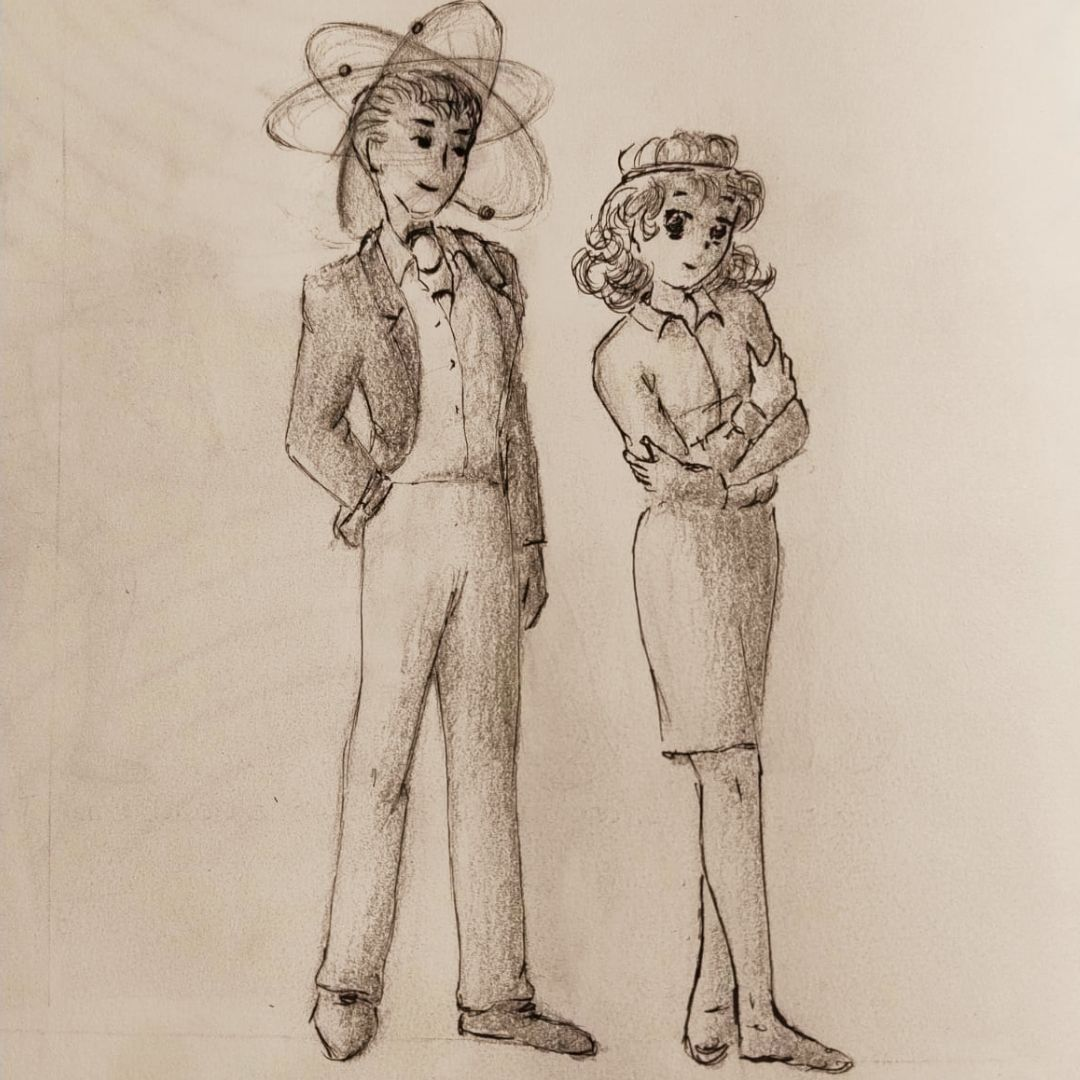
\includegraphics[width=\textwidth]{immagini/cnot_56.jpeg}} % Sostituisci con il nome del file immagine
\end{minipage}
\end{center}
Le sue parole mi attiravano, irresistibili. La sua voce, calma e suadente, scorreva come un fiume tranquillo, facendo scivolare via le paure accumulate nel corso della giornata.

\begin{dialogue}
\speak{Commissario} \enquote{Sai, Caterina, il tuo arrivo qui è davvero straordinario. Persone come te, dotate di una mente brillante e di capacità eccezionali, sono esattamente ciò di cui abbiamo bisogno.}
\end{dialogue}

Le sue parole mi confondevano, e non potei fare a meno di sentirmi valorizzata. In un ambiente dove l'incertezza regnava sovrana e le mie fragilità erano amplificate, il Commissario sembrava rappresentare una boccata d'aria fresca. La sua presenza era rassicurante, e ogni parola pronunciata era un invito a credere che ci fosse un posto per me, un ruolo importante che potevo svolgere.

\begin{dialogue}
\speak{Commissario} \enquote{Non capita spesso di incontrare qualcuno con il tuo potenziale. Hai dimostrato di avere coraggio e determinazione, e non posso fare a meno di rispettare questo. È raro trovare individui che osano sfidare i confini del sistema. Il modo in cui ti sei esposta per proteggere un qubit sconosciuto mi ha colpito.}
\end{dialogue}

Sorpresa dalla sua considerazione, mi sentii quasi fluttuare. Era difficile resistere a un approccio così genuino, e la mia mente iniziò a fantasticare su ciò che avrei potuto realizzare in un mondo governato da una figura così carismatica. Per la prima volta, qualcuno mi vedeva davvero. E mi capiva. Per un attimo ogni dubbio e ogni insicurezza  svanirono.

\begin{dialogue}
\speak{Commissario} \enquote{Immagina di lavorare insieme, di costruire qualcosa di grande. Non voglio solo il tuo aiuto, voglio che tu sia parte di un progetto straordinario. Un esercito di qubit non è solo un'idea; è un sogno che può diventare realtà, e tu potresti essere una delle colonne portanti di questo nuovo ordine.}
\end{dialogue}

Sentii il battito del cuore accelerare, mentre il mio pensiero tornava a quel mondo in cui i fallimenti del passato sembravano finalmente essere superati. Avevo sempre desiderato essere parte di qualcosa di più grande, ma non riuscivo a liberarmi dalla sensazione che ci fosse un costo nascosto in tutto ciò.

\begin{dialogue}
\speak{Caterina} \enquote{Ma come posso fidarmi di te?} domandai. \enquote{Cosa accadrebbe se ti rivelassi troppo? Se ti raccontassi tutto?}
\end{dialogue}

Il Commissario sorrise, un'espressione calda e sincera che sembrava promettere sicurezza.

\begin{dialogue}
\speak{Commissario} \enquote{Io non voglio manipolarti, Caterina. Voglio darti l'opportunità di mostrare al mondo ciò di cui sei capace. La fiducia è fondamentale, e ti assicuro che non ho intenzione di danneggiarti. Credimi, ho bisogno di te.}
\end{dialogue}

Sentivo la tensione svanire, mentre la mia mente veniva avvolta dalle sue parole affascinanti. Eppure, mentre mi lasciavo sedurre dal suo discorso, un ricordo tornò a galla. Le parole del mio fidanzato, che mi esortava a non aprirmi a chiunque, a mantenere le mie difese.

In quel momento, mi resi conto che stavo per rivelargli della presenza di Laura e del nostro legame dovuto forse al Noemografo. Decisi di fermarmi. L'idea di fidarmi completamente di un estraneo, per quanto affascinante, mi turbava profondamente.

Con un velo di determinazione, cercai di mantenere un po' di riserbo, ma lo feci con grazia.

\begin{dialogue}
\speak{Caterina} \enquote{Grazie per le tue parole, ma ho bisogno di tempo per riflettere,} dissi, cercando di mascherare il conflitto che si stava formando nel mio cuore. Il commissario però continuava a pormi domande, prima semplici e dirette, poi più complesse ed incrociate, correvo il rischio di contraddirmi o di svelarmi.
\end{dialogue}

\section{La Fuga e la Trappola}

Decisi allora di cambiare approccio. Dovevo fingere di cedere, di lasciarmi sedurre dal Commissario. Iniziai a sorridergli, annuendo alle sue parole e lasciandomi trasportare dal suo discorso. Ogni tanto rispondevo con un cenno di assenso, un sussurro, facendogli credere di essere totalmente presa da lui. Sapevo che, se volevo avere una possibilità di fuga, dovevo essere convincente.

Il Commissario continuava a parlare, le sue parole erano suadenti, piene di fascino e di promesse.

\begin{dialogue}
\speak{Commissario} \enquote{Sai, Caterina, un giorno potresti avere un ruolo importante qui. Questo mondo ha bisogno di risorse come te, e con qualcuno come me al comando, potremmo realizzare grandi cose.}
\end{dialogue}

Il suo tono era quello di un leader, di un visionario che credeva in un futuro grandioso, e per un momento mi chiesi se non avesse davvero un piano così ambizioso.
Chiusi gli occhi e mi avvicinai. Le mie labbra erano appena dischiuse, sperando che lui ricambiasse. Ci baciammo delicatamente ma prima che i nostri corpi si scaldassero gli chiesi di lasciari il tempo per spogliarmi. Con galanteria, il Commissario uscì dalla stanza, lasciandomi sola. Ero riuscita nel mio intento, e questa era l'occasione che aspettavo per fuggire,  ma quando ci provai  mi ritrovai immobilizzata da una forza invisibile che mi tratteneva.

\begin{dialogue}
\speak{Commissario} \enquote{Mi avevi quasi convinto} disse, con un sorriso tranquillo.
\end{dialogue}

Prima che potessi reagire, fece un cenno e, quasi come per magia, una rete di particelle luminescenti cominciò a formarsi intorno a me. Cercai di muovermi, ma i miei polsi e caviglie furono bloccati in una morsa invisibile, un campo di energia mi stava immobilizzando.

\begin{dialogue}
\speak{Caterina} \enquote{Cosa stai facendo?} chiesi, cercando di mantenere la calma, ma la voce mi tremava leggermente.
\end{dialogue}

Il Commissario si avvicinò, e con un'espressione impassibile spiegò:

\begin{dialogue}
\speak{Commissario} \enquote{Non pensavi davvero di poter sfuggire, vero? Questa è la mia \textit{Ion Trap}, una trappola  che immobilizza ogni particella, anche le più ribelli,  all'interno del suo campo.}
\end{dialogue}

Una scarica elettrica mi percorse braccia e gambe, serrando ogni movimento. Ero impotente. Il cuore mi batteva forte mentre la consapevolezza della mia cattività mi calava addosso. Il Commissario mi fissava, implacabile. Percepii in lui una crudeltà che era stata nascosta dietro le sue lusinghe.

\begin{dialogue}
\speak{Commissario} \enquote{Non sei altro che una pedina in questo gioco. Pensavi di poter giocare con me?  Ora vedremo chi di noi ha il vero potere.}
\end{dialogue}

Abbassai lo sguardo, cercando di non mostrare il mio terrore. Sapevo che ora sarei stata completamente in balia del Commissario, e ogni speranza di fuga sembrava svanita in quel campo di ioni che mi imprigionava. Non restava che il silenzio e la stretta implacabile di quel campo di ioni.
